\documentclass[12pt,english]{article}
\usepackage{mathptmx}

\usepackage{color}
\usepackage[dvipsnames]{xcolor}
\definecolor{darkblue}{RGB}{0.,0.,139.}

\usepackage[top=1in, bottom=1in, left=1in, right=1in]{geometry}

\usepackage{amsmath}
\usepackage{amstext}
\usepackage{amssymb}
\usepackage{setspace}
\usepackage{lipsum}

\usepackage{natbib}
\usepackage{url}
\usepackage{booktabs}
\usepackage[flushleft]{threeparttable}
\usepackage{graphicx}
\usepackage[english]{babel}
\usepackage{pdflscape}
\usepackage[unicode=true,pdfusetitle,
 bookmarks=true,bookmarksnumbered=false,bookmarksopen=false,
 breaklinks=true,pdfborder={0 0 0},backref=false,
 colorlinks,citecolor=black,filecolor=black,
 linkcolor=black,urlcolor=black]
 {hyperref}
\usepackage[all]{hypcap} % Links point to top of image, builds on hyperref
\usepackage{breakurl}    % Allows urls to wrap, including hyperref

\linespread{2}

\begin{document}

\begin{singlespace}
\title{A Glimpse into the English Premier League}
\end{singlespace}

\author{Travis Richardson\thanks{Department of Health and Exercise Science, University of Oklahoma.\
E-mail~address:~\href{mailto:student.name@ou.edu}{twrichardson@ou.edu}}}

% \date{\today}
\date{April 16, 2019}

\maketitle

\begin{abstract}
\begin{doublespace}
The English Premier League is the most popular league in the entire world, with a TV viewing audience of about 4.7 billion people. A better understanding of such a prominent league would lead yo better coaching decisions, better articles and write-ups, and most importantly (to certain people) better gambling odds \citep{ulmer}. In this paper, a statistically significant (R-squared:  0.9188), 33-variable multiple regression model, as well as a statistically significant (R-squared:  0.9237), 34-variable multiple regression model are used to predict goals and wins in a single English Premier League season. Additionally, for better understanding of how the teams in the English Premier League differentiate, a linear regression is ran in order to see the differences in the top teams, the middle of the pack teams, and the bottom dwellers of the past 12 seasons of the English Premier League. Additional visuals are presented for better perspective on important measures such as: correlation between goals and wins and then how long each of the 39 teams in the data set of been in the EPL for the last 12 years. Full results will later be added to the abstract
\end{doublespace}

\end{abstract}
\vfill{}


\pagebreak{}


\section{Introduction}\label{sec:intro}
\begin{Introduction}


\begin{doublespace}
As mentioned, the English Premier League is one of the most popular leagues in the world with over 4.7 billion views each year and an average of 12 million viewers per game. With the introduction of data analytics in sports, for years now people have been trying to predict scores and outcomes of games using machine learning and multiple regression models. However, in 2010 the famous Paul the Octopus put all models to shame when it predicted a perfect eight out of eight matches correctly. Whether Paul has dumb luck or is a soccer genius, the feeling of knowing less about the beautiful game that an octopus left a sour taste in many analysts mouths. For this reason, the first part of this paper discusses the prediction of goals and wins for single English Premier League seasons. "Predicting" is being used in a loose sense, however, the games have already been played and the data is set so the predictive models in this research are comparing fit to see how the models match up to the actual outcomes. Having a model with high correlation and fit will allow for future research to lead into predictive modeling in order to truly predict future seasons goal and win totals. Predictive modeling can lead to better coaching tactics, proper journalism, and more accurate betting odds. Coaches can benefit from predictive modeling by having an understanding of their team and looking into why they are predicted to only score a certain amount of goals or only win a certain amount of games. What is the team lacking or what do they need to focus on that better teams are doing, are questions managers could look at. Every sports fan gets excited for the predictions for each season, typically to be let down when their team finishes in 4th place (like always). Predictive modeling can help journalism in ways as to have proper and accurate assumptions leading to fans trusting that specific news source. The journal with the most accurate predictions would quickly become a fan favorite. This leads to predictive modeling providing more accurate betting odds. If a company giving out betting odds has extremely accurate goal and outcome predictions for single games or seasons, they would end up having to pay out less money. Vice versa, with better prediction modeling, gamblers will feel as they have better chances of winning big.\\
\indent The next part of this paper will discuss the differentiation between top teams, middle of the pack teams, and lower tier English Premier League teams. In this research, top tier teams are defined as any team that has been in the English Premier League for at least 10 of the last 12 seasons (12). Middle of the pack teams are defined as being in between 9 and 4 seasons (15). Then lower tier teams are defined as having from 3 down to only 1 year in the Premier League (12). In European sports, quite the opposite of American sports, there are actually consequences to performing poorly during the season and rewards for performing well. The bottom three teams each year get relegated to a lower division and the top four teams qualify for the most prestigious tournament in the world, the UEFA Champions League. Being relegated or in the champions league determines a very big difference in income for a team \citep{oberstone}. Understanding the differences in these three categories of teams could allow for teams to realize possible stats and play types they are not performing properly and be able to adapt and become a top tier team. 
\end{doublespace}
\end{Introduction}


\section{Literature Review}\label{sec:litreview}
\begin{Literature Review}
\begin{doublespace}

Although no analyst will ever be able to compare to the outstanding predictions of Paul the Octopus, there are still many predictive models and research papers done to try and perfect predicting scores and outcomes of games. Three known articles about predicting match results in  the English Premier League and the World cup that will be used in this paper are from the works of Ben Ulmer & Matthew Fernandez, Francisco Louzada, Adriano K. Suzuki & Luis E. B. Salasar, and Andreas Groll, Gunther Schauberger & Gerhard Tutz. Ulmer and Fernandez predict the results of English Premier League games using artificial intelligence and machine learning algorithms. They look into historical data and then the current teams form while using five different classifiers to predict win, loss or draw. However, from those five classifiers, their best error rates were only .48 and .50. This article emphasizes the importance of predictive modeling for gambling and coaching improvements \citep{ulmer}.\\
\indent In the next paper being examined, Louzda, Suzuki, and Salasar predict outcomes of the English Premier League as well, but with a focus on predicting who the champion will be. They are also interested in looking into "the end result of a match, the chance of a team to be qualified for a specific tournament, the chance of being relegated, the best attack, the best defense," \citep{louzada}. To predict these outcomes, the authors are estimating average goals scored by assuming goals scored by each team follows a univariate Poisson distribution. The estimation of goals in Louzda's paper correlates with the prediction of goals for this paper at hand, however, the model in this paper uses 34 variables, while Louzda only uses 5 covariates; which could make a difference.\\
\indent The final paper being examined in regard to prediction of matches, by Groll, Schauberger, and Tutz looks into predicting World Cup 2014 matches using Poisson regression. Although not about the English Premier League, the authors try to predict World Cup success based on previous World Cup performances, which is similar to predictions made in this paper. The final predictions in both the models after being fitted and investigated favored Germany as the winner; which this ended up becoming true \citep{groll}.\\
\indent The other two articles being examined are from the works of Joel Oberstone and Jaime Araya & Paul Larkin. Joel Oberstone's article "Differentiating the Top English Premier League Football Clubs from the Rest of the Pack: Identifying the Keys to Success" was a large foundation of why this paper came about. The questions of what distinguishes the best teams from all the rest was a thought that had been in the air for awhile and I wanted to help answer it. Oberstone looks into 24 "pitch actions" collected during the 2007/2008 season \citep{oberstone}. The author separates the teams from that season into 3 groups, the top four teams, the middle twelve, and the bottom four teams. First, a regression was done to determine six statistically significant factors that led to the club's ultimate success in that season. The six factors were: Percent Goals scored outside box, Percent of goals to shots, Number of yellow cards, Ratio of short to long passes, Number of total crosses, and Average goals conceded per game. Secondly, the 24 variables used in the one-way ANOVA determine that their are thirteen actions that are statistically significant that separate the three groups from one another.\\
\indent The final paper to be examined was "Key performance variables between the top 10 and bottom 10 teams in the English Premier League 2012/13 season" by Jaime Araya and Paul Larkin. As the title suggests, Araya and LArkin are examining what variables are different between the teams that finish in the top 10 of the English Premier League and then the teams that finsih in the bottom 10. They state that, "research has indicated that possession, shots at goal, and goals scored are key performance indicators for successful football teams. There is however, a lack of understanding of other potential attacking and defensive performance variables that may contribute to successful performance" \citep{araya}. The authors look at in-game statistics from 380 games from the 2012/2013 season. Their findings show that top tier teams tend to have more possession (p>.01), have a lot more shots (p>.01), score more from inside the 18-yard box (p=.02), have shorter passes, and then score more in open play. Basically, to be a top 10 team in the English Premier League, Araya and Larkin discovered teams need to "keep possession of the ball via short passes, with the attempt to penetrate the opposition defence to have a shot at goal from inside the 18-yard box" \citep{araya}.

\end{doublespace}
\end{Literature Review}


\section{Data}\label{sec:data}
\begin{Data}
\begin{doublespace}


The primary data source for this research is English Premier League team statistics for the 2006/2007 season through the 2017/2018 seasons. This dataset was found on Kaggle. The data is set up, starting with the 2006/2007 season, by the place each team finished. Manchester United won the 2006/2007 season followed by Chelsea, Liverpool, and Arsenal; after these teams the rest of the league, by position, is ordered. Once the twenty teams from that season are listed, the next season starts with the league leader, and this carries on all the way through to the 20017/2018 season. There are a total of 35 variables used in the data that are also used in regressions for this paper, those variables include: wins, losses, goals, total.yel.card, total.red.card,	total.scoring.att,	ontarget.scoring.att,	hit.woodwork, att.hd.goal,	att.pen.goal,	att.freekick.goal,	att.ibox.goal,	att.obox.goal,	goal.fastbreak,	total.offside,	clean.sheet,	goals.conceded,	saves,	outfielder.block,	interception,	total.tackle,	last.man.tackle,	total.clearance	own.goals,	penalty.conceded,	pen.goals.conceded,	total.pass,	total.long.balls,	total.cross,	corner.taken,	touches,	clearance.off.line,	penalty.save,	total.high.claim,	punches. For non-soccer fans, some of these variables might be rather confusing, so a few of the variables will be expanded upon. Total.scoring.attempt is a fancy way of saying total number of shots. Att.hd.goal is a header being scored, att.ibox.goal and att.obox.goal are scoring from inside or outside the box. Outfielder.block is when a field player (not the keeper) blocks a shot. Penalty.conceded is when the team fouls someone and gives up a penalty and then penalty.goal.conceded is when they are scored on after giving up the foul. Total.high.claim is when the keeper jumps up and takes the ball over top other players. Most other variables seem rather obvious, even for a non-soccer fan. \\
\indent The original dataset was rather clean, so no true cleaning of the data had to be done. However, a few extra variables were added based on other given variables to help with correlation and regressions. Since teams are disbursed throughout separate seasons, an extra "Team" variable was added to show the 39 unique teams that have been in the English Premier League in the last twelve seasons. From this list of teams, I represented how many years they have been in the league in the past twelve years with "Years in EPL". "Total Goals" and "Total Wins" were added to show the total amount of wins and goals they have had in the last twelve seasons. "Avg WPS" represents the average amount of wins each team had per season and then "Avg.goals" then represents the average amount of goals each team had per season.\\
\indent For one package in R, Corrplot, to create the needed plot to represent correlation, an extra data source was created to make everything into numeric data. In the original dataset, most variables were numeric, however, when trying to change just a few, I was unable to do so. This led to making a new data set and deleting out the unwanted variables in order to run the specific correlation. However, this source was only used for the one package a correlation. 

\end{doublespace}
\end{Data}


\section{Empirical Methods and Research Findings}\label{sec:methods}
While my approach explores a number of different approaches, the primary empirical model can be depicted in the following equation:

\begin{equation}
\begin{align*}
    
\label{eq:1}
Y_{goalfit}= \alpha_{-4.17} + X_{1}{wins}+X_{2}{losses}+X_{3}{total.yel.card}+X_{4}{total.red.card}+X_{5}{total.scoring.att}+X_{6}{ontarget.scoring.att}+X_{7}{hit.woodwork}+X.{8}{total.offside}+X_{9}{clean.sheet}+X_{10}{goals.conceded}+X_{11}{saves}+X_{12}{outfielder.block}+X_{13}{interception}+X_{14}{total.tackle}+X_{15}{last.man.tackle}+X_{16}{total.clearance}+X_{17}{own.goals}+X_{18}{penalty.conceded}+X_{19}{pen.goals.conceded}+X_{20}{total.pass}+X_{21}{total.long.balls}+X_{22}{total.cross}+X_{23}{corner.taken}+X_{24}{touches}+X_{25}{clearance.off.line}+X_{26}{penalty.save}+X_{27}{total.high.claim}+X_{28}{punches}


\end{align*}
\end{equation}
where $Y_{goalfit}$ is a continuous dependent variable for all 28 independent variables in the dataset. The 28 variables, including: wins, losses, total yellow cards, total red cards, total shots, total shots on target, shots that hit the woodwork, total offsides, clean sheets, goals conceded, saves, outfielder blocks, interceptions, total tackles, last man tackles, total clearances, own goals, penalties conceded, penalty goals conceded, total passes, total long balls, corners taken, touches, clearances off the line, penalty saves, total high claims, and punches by the keeper. These are the independent variables that allow for the dependent variable "Goals" to be predicted upon. \\
\indent Although this equation is a very important part of this research, it is not the only steps taken to understand the English Premier League on a deeper level. The first step in this research was to understand the basic correlations of stats and variables given from the data set. Goals and wins were correlated against one another to look into how important goals are to represent wins. As assumed, these two variables were extremely positively correlated at .97. The R produced graph will be Graph 1 in the tables and graphs section at the end of the paper. This strong correlation indicates that the more goals scored by a team, the more likely they are to win. This conclusion brought another question, however, that question will be discussed later. After looking into just the correlation between goals and wins, a total of 19 variables were then correlated against one another. These variables included: wins, losses, goals, yellow, red, shots, woodwork, InsideBox, OutsideBox, Offside, clean sheet, goals conceded, saves, interception, clearances,	own goals, passes, longballs, and touches. Again, this correlation plot will be Graph 2 in the graph and table section at the end of the paper. Some interesting conclusions based on the correlations are: wins is highly correlated (.7) with both touches and passes; these two variables are what make up possession in a simple definition. This explains that possession is very highly correlated with wins. In simpler terms the team with more of the ball is going to win more. Another finding is that clean sheets and goals are correlated at .57 indicating that teams that do not allow goals the be scored on them are more likely to score on the opposing team. This can be attributed to, assuming that the team had a clean sheet because their defense was playing well would lead to the offense having the ball more and having more opportunities to score. One last finding that will be discussed is that clearances and passes are negatively correlated at .57. This is most likely due to the fact that clearances are more a last ditch effort from the defense in order to get he ball as far away from their goal as possible, leading to the team not passing out of the back. The more clearances a team has, the less passes the defense would be making. This is indicative of the negative correlation. \\
\indent Following the correlation steps, next was to predict goals and wins based on the variables from the data set. The equation above is the equation used to predict goals. The equation used to predict wins is exactly the same, except wins and losses are substituted for goals. The R-Squared value for the goal prediction equation is .91 and the p-value is below .001. These two values represent that the equation is very representative and is significant. The equation for predicting wins has an R-squared value of .91 and a p-value of below .001 as well. Again, this indicated the equation has a 91 percent chance of predicting the score correctly and is significant. \\
\indent The next stage of the research came from the goals and wins correlation. As mentioned, that graph made another question come to mind. In the graph, there seems to be a very defined group of teams that are high above the rest. So the question of how long each team had been in the English Premier League for the past 12 seasons occurred. The graph for this will be Graph 3. Making a bar chart of time in the English Premier League showed three obvious and distinct groups. This is where the Top-Tier, Middle-of-the-Pack, and Lower-Tier team groups came about. Once the teams were separated into three distinct groups, the final section of the research was conducted; How do the three groups differ from each other and why might those differences occur.\\
\indent To compare the three groups, an experience tier was created in R to separate the groups. Then linear regressions were ran comparing 12 different variables against the different groups. The variables comparing the three groups were: Shots, shots on target, goals from fast breaks, total offsides, interceptions, total tackles, outfielder blocks, total clearances, total passes, total long balls, total crosses, and total touches. Some of the more interesting variables will be discussed. \\
\indent For both shots and shots on target, the Top-Tier teams were far ahead of the other two groups. This is pretty obvious because the best teams will be scoring the most which means they will be taking the most shots. For fastbreak goals, I assumed lower level teams would actually have more than the higher tier teams; this is based off the fact that the low-tier teams play the most through balls and middle-of-the pack teams are not far behind. However, the top-tier teams scoring more fastbreaks correlates with the top-tier teams also having the most offsides. The players are eager to get in behind the defense and score. Interceptions was interesting; middle-of-the pack teams actually had the highest amount of interceptions, then top-tier, then low-tier. This could be due to the middle teams being more aggressive to get the ball, but then shortly losing possession after. Outfielder block (any player beside the keeper making a block) is actually highest for low-tier teams and then next for the middle teams. This is most likely due to high-tier teams being able to take more shots and the other teams having to block them so the shots are not on target. This is a similar explanation to total clearance. Again, the lower teams have a higher amount of clearances, most likely because the high-tier teams are on offense longer and the worse teams have to kick the ball away more often. Total passes and total touches is as assumed; the higher tiered teams are far and above the others. These assumptions are not based on facts, strictly personal bias and opinion. 



\section{Conclusion}\label{sec:Conclusion}
The main results for this research aren't perfectly straight forward. Since there were three steps in this report; correlation, prediction, and comparison, the findings and concluding comments represent those steps. \\
\indent Correlation: The correlation section represents that wins and goals are very highly correlated. This led to the correlation table to compare even more variables. The graph shows that a few interesting findings, as discussed before, such as, touches and passes being highly correlated with wins. Clean sheets and goals were highly correlated, representing the need for a proper defense to gain advantage on offense. And lastly, clearances and passes were negatively correlated. This leads to the assumption that certain defenses need to pass the ball out of the back more instead of going for clearances. Since passing is highly correlated with wins, clearing the ball every time does not seem like the best tactic.  \\
\indent Prediction: In the prediction section goals and wins were dependent variables used to see if all the other independent variables could accurately predict the outcomes. For both goals and wins, the R-squared and p-values were very indicative that the linear models worked and could accurately predict the two dependent variables. \\
\indent Comparison: Possibly the most important part of the research was comparing the three groups. Top-Tier, Middle-of-the-pack, and lower-tier teams were the three distinctive groups. The conclusions made based on the linear models ran were basically that the top-tier teams have more shots, more shots on target, more passes and touches (possession), more fastbreak goals, and more crosses. These statistics can be shown that the top-tier teams control the game with more shots and possesion and are also more athletic in their ability to get fast breaks and and cross the ball. The middle-of-the-pack and low-tier teams were had higher averages in interceptions, outfielder blocks, clearances, and long balls. All of these attributes have negative correlations involved with them. The lower tiered teams average more interceptions because they are aggressively trying to gain possession but once they have possession they can not keep the ball and have to go for another interception. Outfielder blocks and clearances are similar in thinking that the defenses for the lower teams are working harder in order to keep from getting scored on. And having more long ball passes can show a desperation to try yo get in behind the better defense. \\
\indent Overall, this research paper represents that Top-Tier teams are considered top-tier based on how many years they have been in the league. Not being relegated at all or very few times shows the level of ability to control a game through possession and shots. This research can be used by coaches or gamblers to understand that not forcing the ball through clearances and long balls, keeping the ball with short passes and many touches, and taking more and better shots is the way to understand the difference between Top-Tier teams and the rest. 



\vfill
\pagebreak{}
\begin{spacing}{1.0}
\bibliographystyle{jpe}
\bibliography{References.bib}
\addcontentsline{toc}{section}{References}
\end{spacing}

\vfill
\pagebreak{}
\clearpage

%========================================
% Graphs and Tables 
%========================================
\section*{Graphs and Tables}\label{sec:figTables}
\addcontentsline{toc}{section}{Graphs and Tables}
%----------------------------------------
% Figure 1
%----------------------------------------
\begin{figure}[ht]
\centering
\bigskip{}
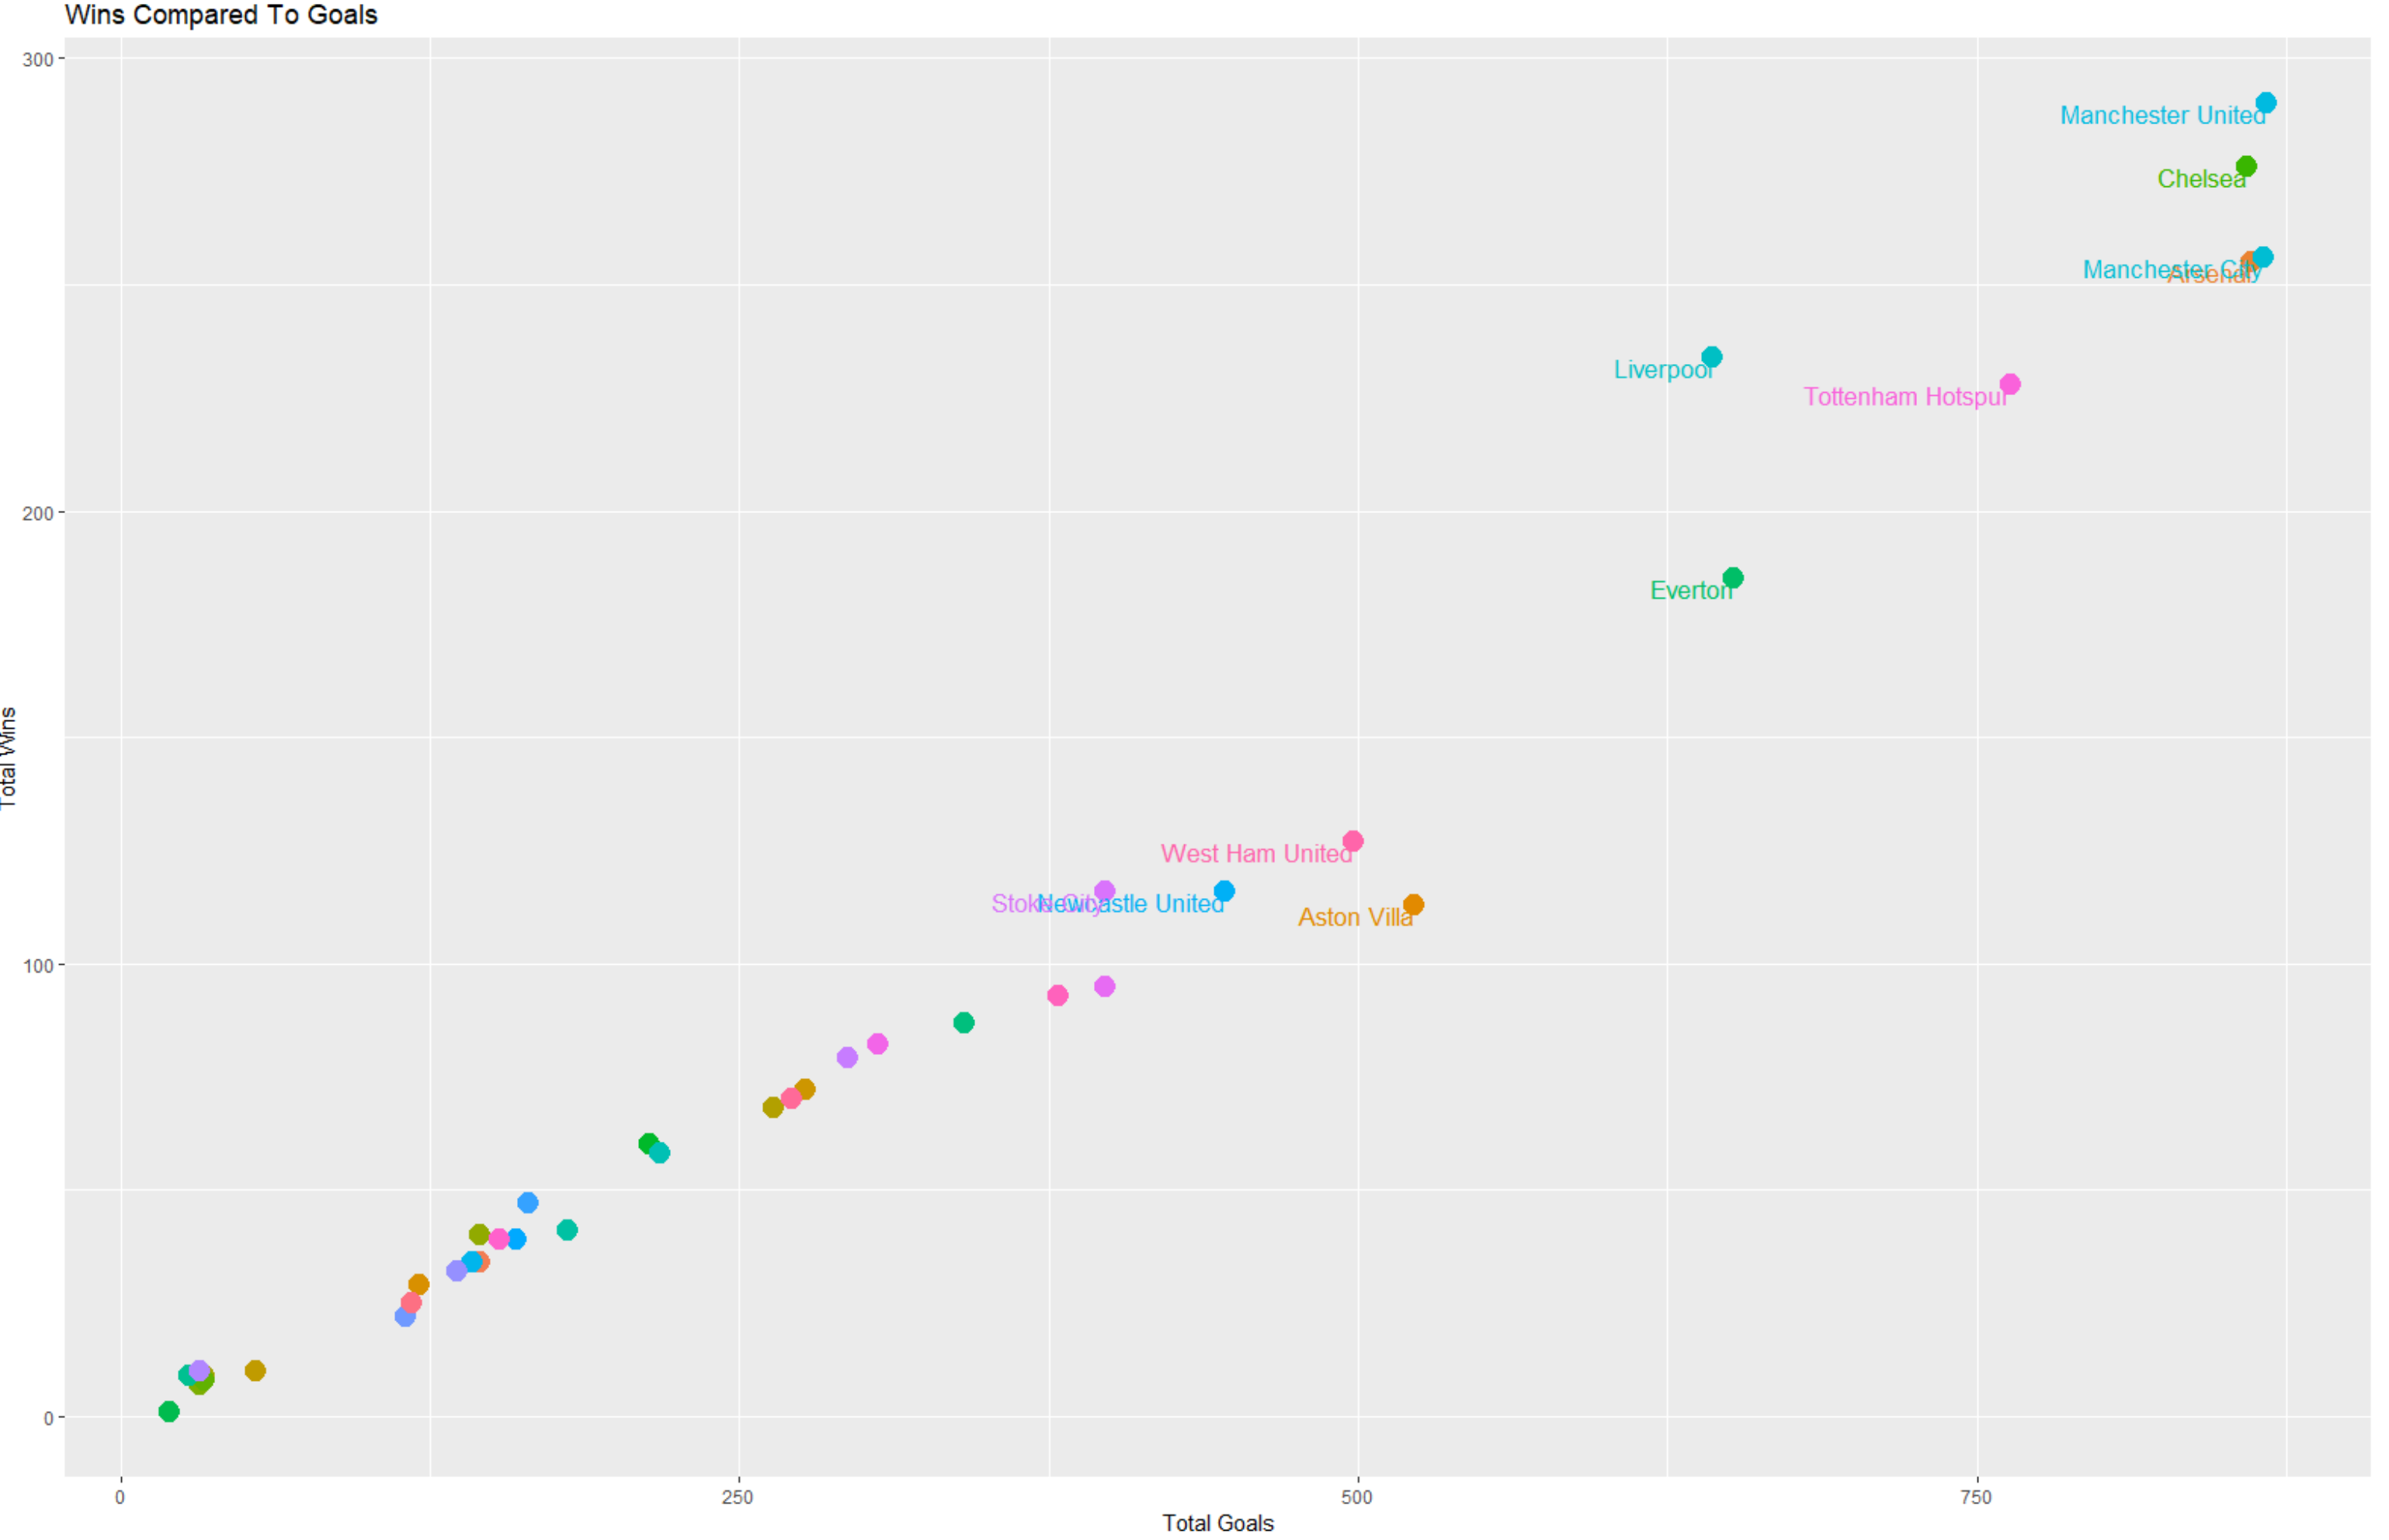
\includegraphics[width=1.2\linewidth]{Correlation.PNG}
\caption{Correlation Goals and Wins}
\label{fig:fig1}
\end{figure}

\begin{figure}[ht]
\centering
\bigskip{}
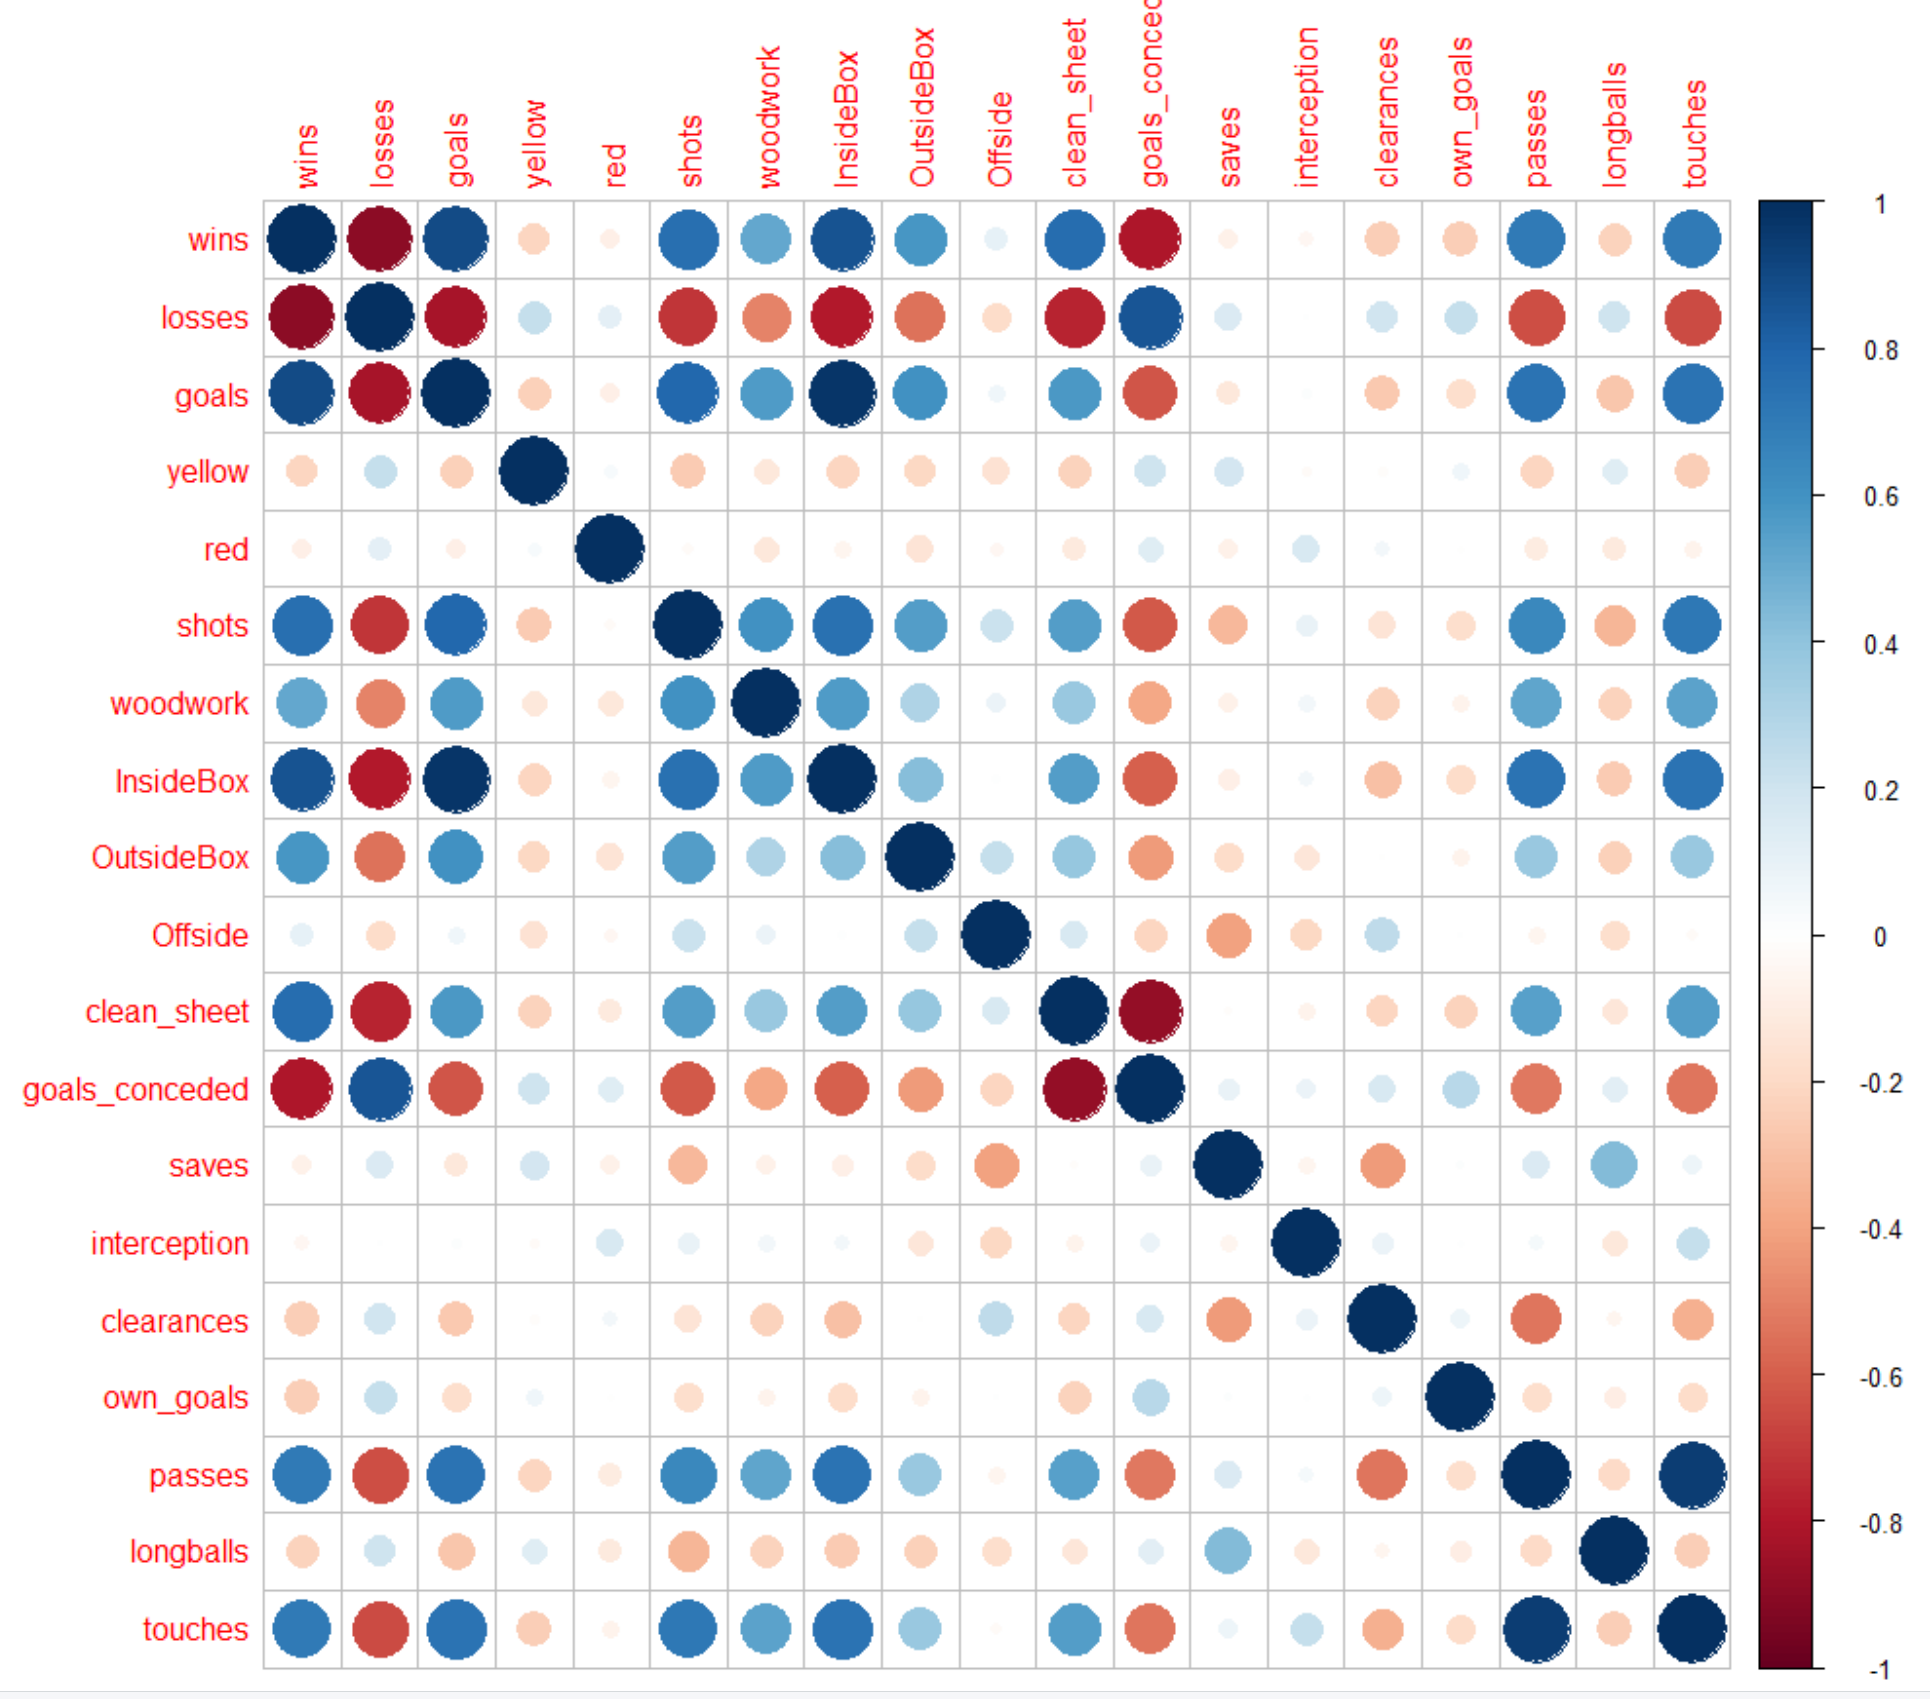
\includegraphics[width=1.2\linewidth]{Circles.PNG}
\caption{Correlation of 19 variables}
\label{fig:fig1}
\end{figure}

\begin{figure}[ht]
\centering
\bigskip{}
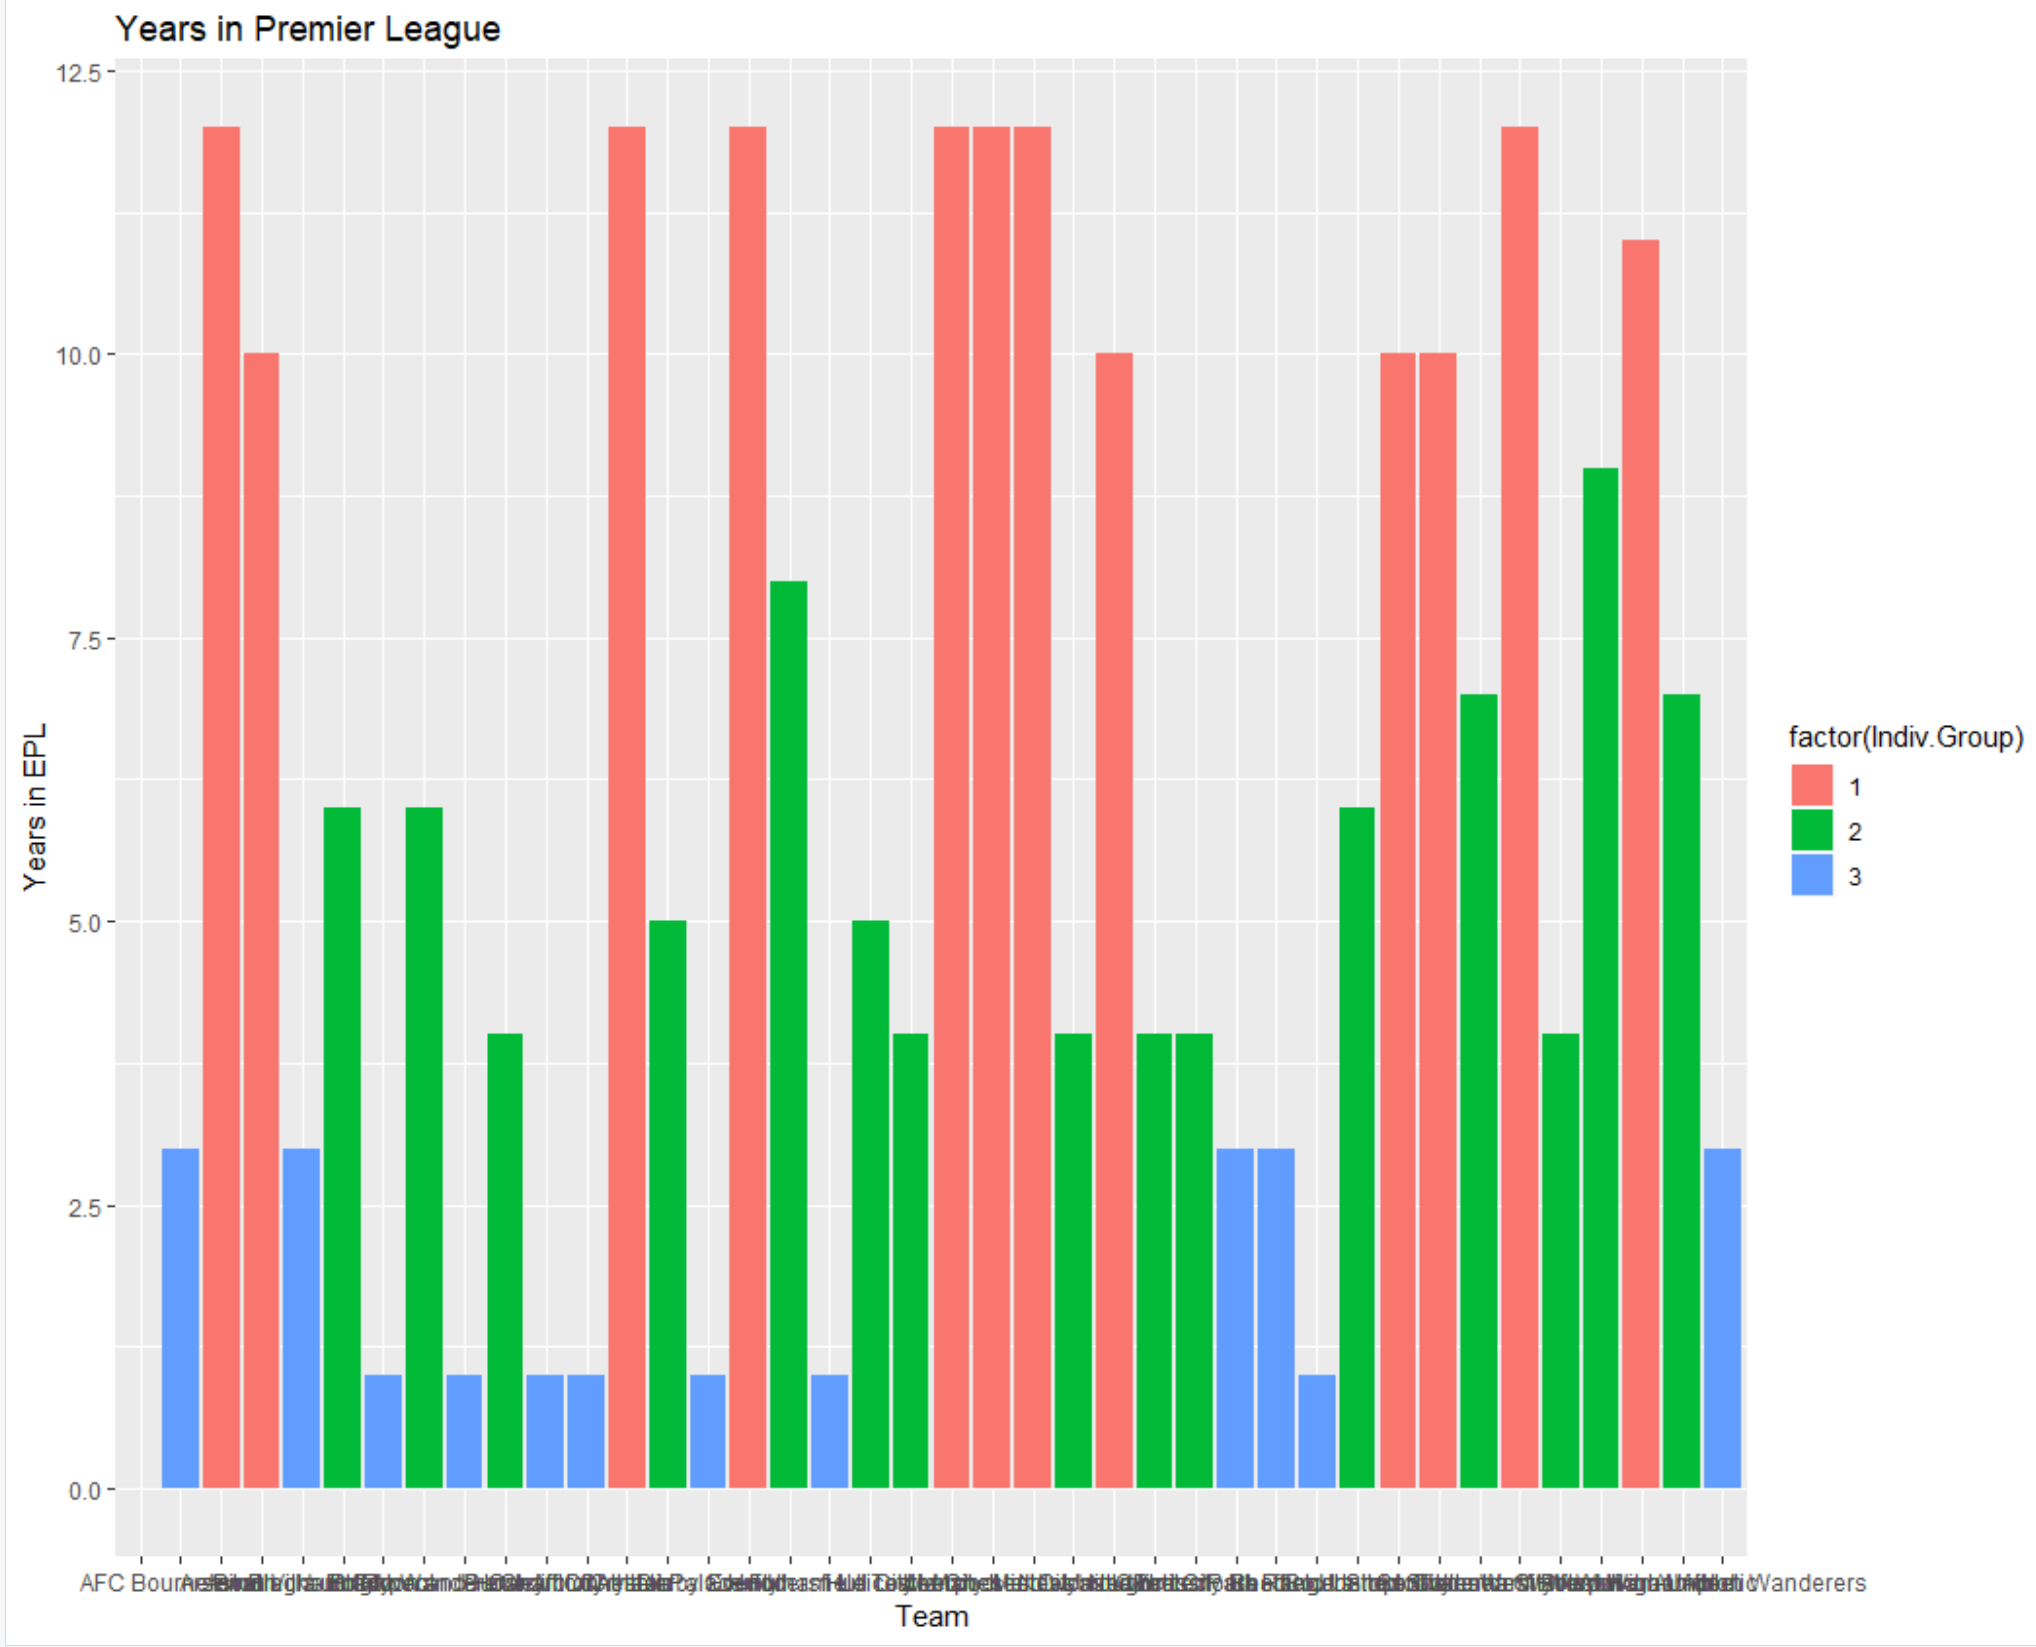
\includegraphics[width=1.2\linewidth]{Groups.PNG}
\caption{Years in Premier League separated by group}
\label{fig:fig1}
\end{figure}

\begin{figure}[ht]
\centering
\bigskip{}
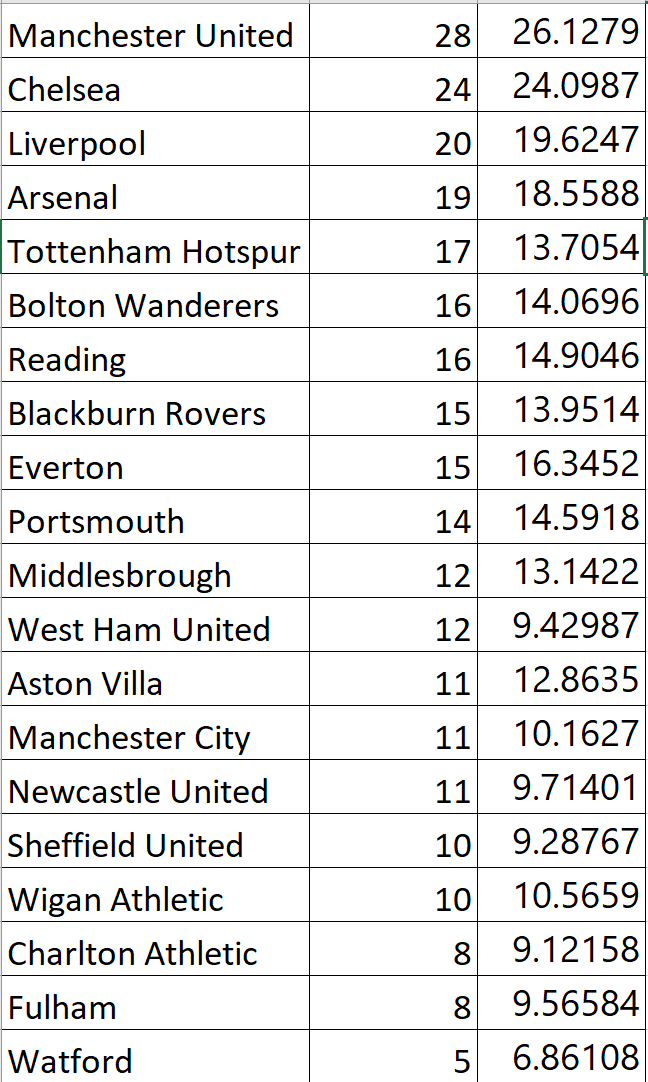
\includegraphics[width=.7\linewidth]{Pred Wins.PNG}
\caption{First season: Actual wins vs predicted wins}
\label{fig:fig1}
\end{figure}

\begin{figure}[ht]
\centering
\bigskip{}
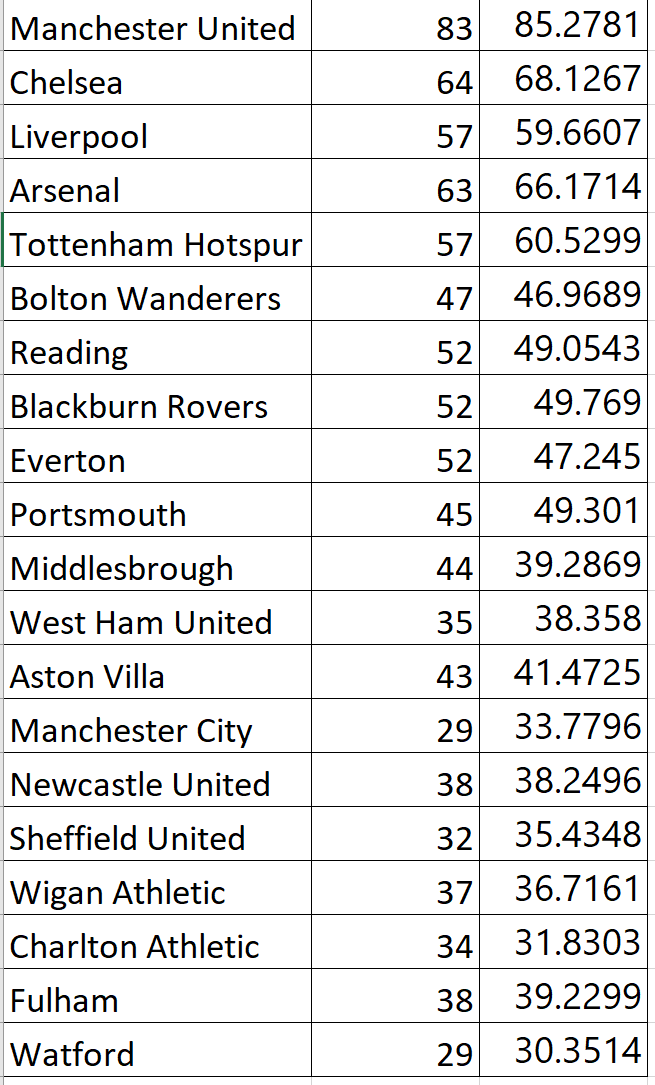
\includegraphics[width=.7\linewidth]{Pred Goals.PNG}
\caption{First Season: Actual goals vs predicted goals}
\label{fig:fig1}
\end{figure}

\bibliographystyle{plain}
\bibliographystyle{bibliography}
\end{document}